\documentclass{report}



\usepackage{amsmath}
\usepackage{amssymb}
\usepackage{graphicx}
\usepackage{dsfont}
\usepackage{pgfplots}
\usepackage{caption}

\usepackage{algorithm}
\usepackage{algpseudocode}




\begin{document}
\begin{figure}[ht]
\centering
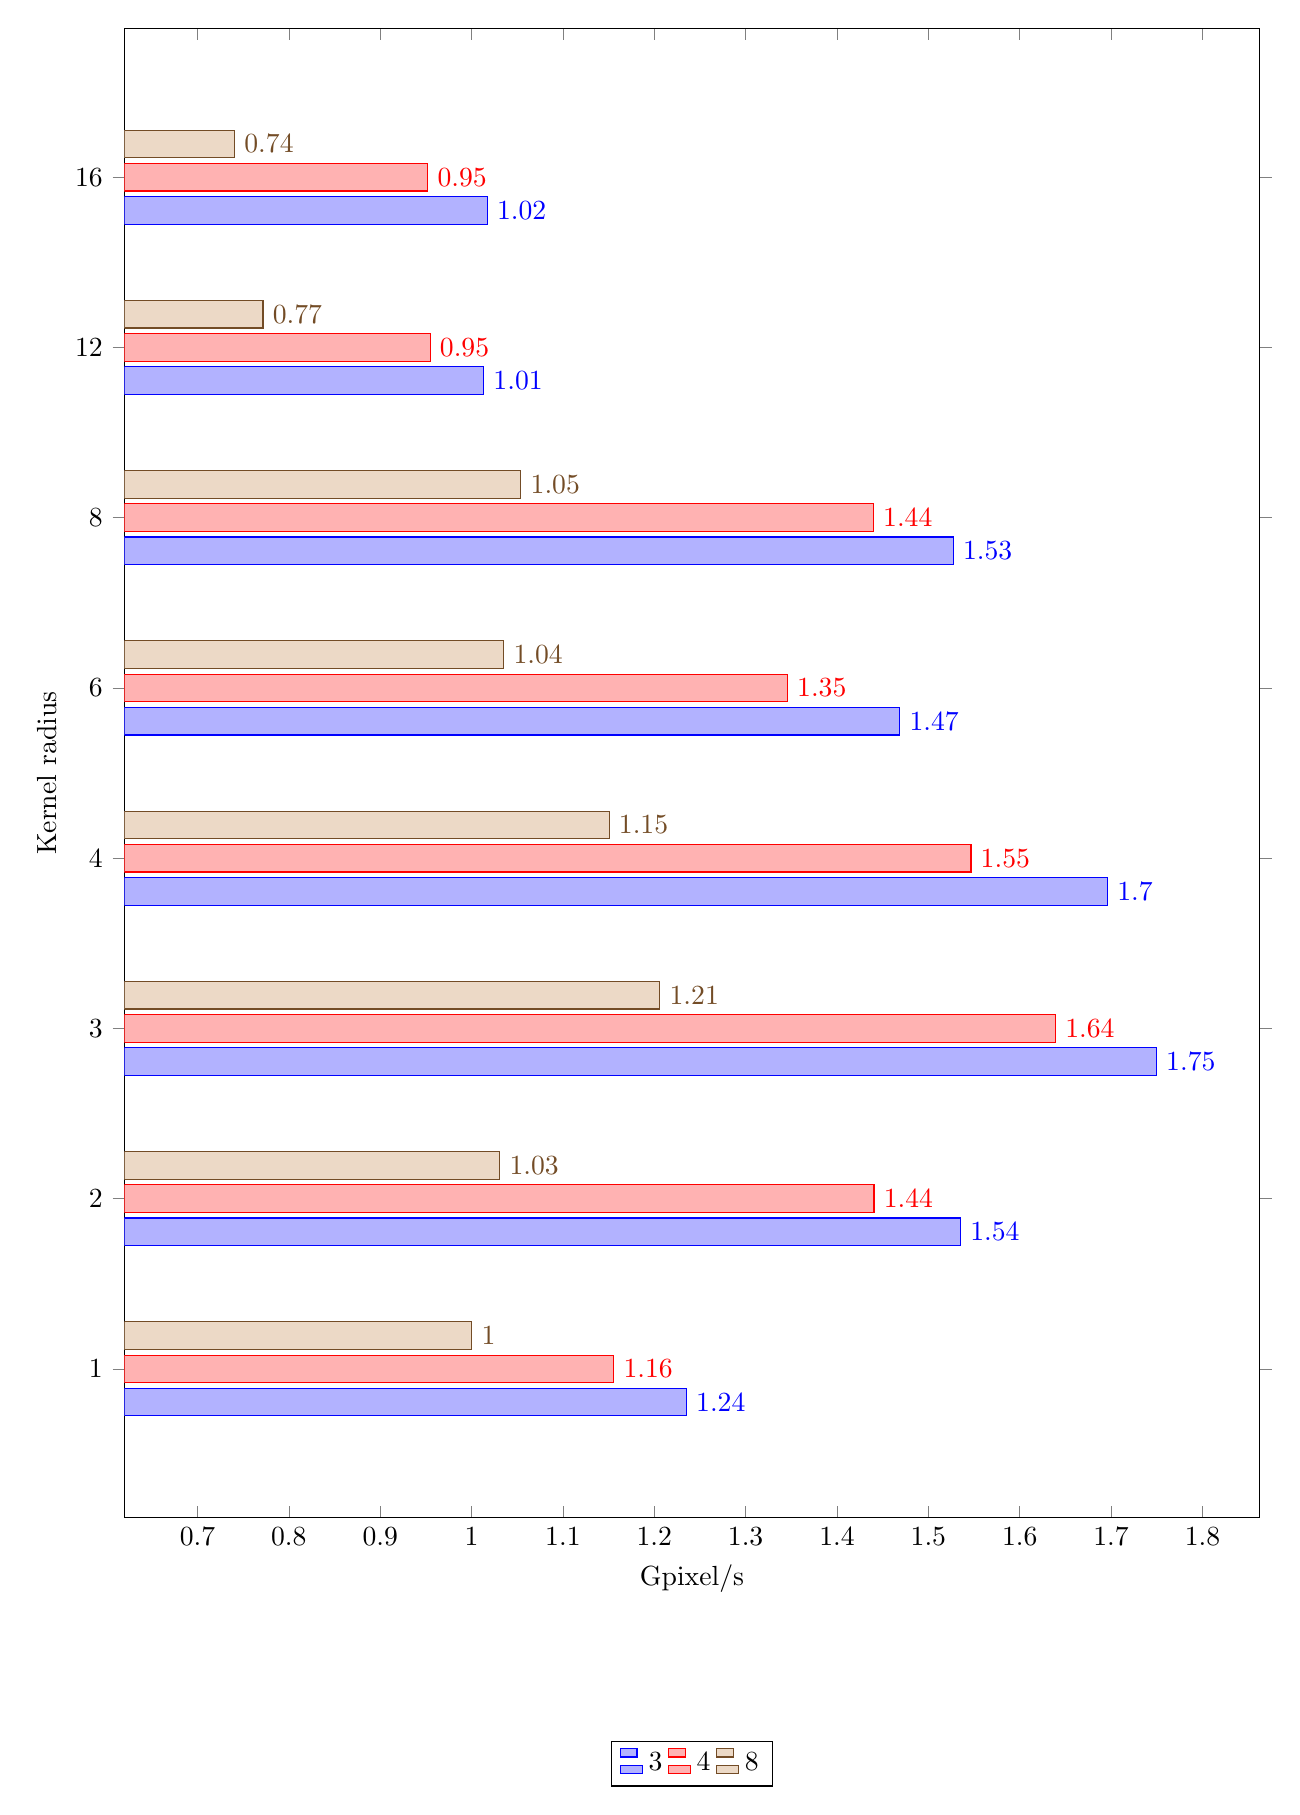
\begin{tikzpicture} 
\begin{axis}[ 
	xbar, 
	xmin=0.62, 
	width=16cm, 
	height=20.5cm, 
	enlarge y limits=0.125, 
	xlabel={Gpixel/s}, 
	ylabel={Kernel radius}, 
	symbolic y coords={1,2,3,4,6,8,12,16}, 
	ytick=data, 
	nodes near coords, 
	nodes near coords align={horizontal}, 
	legend style={at={(0.5,-0.15)}, anchor=north, legend columns=-1}, 
	] 
	
  \addplot coordinates {(1.23517,1) (1.53526,2) (1.74967,3) (1.69605,4) (1.46878,6) (1.52733,8) (1.01331,12) (1.01721,16)};
  \addplot coordinates {(1.15571,1) (1.44051,2) (1.63918,3) (1.54663,4) (1.34572,6) (1.43985,8) (0.95468,12) (0.95204,16)};
  \addplot coordinates {(1.00025,1) (1.03096,2) (1.20613,3) (1.15062,4) (1.03529,6) (1.05403,8) (0.77176,12) (0.74066,16)};

 
 



\legend{3,4,8} 

\end{axis} 
\end{tikzpicture}
\end{figure}

\end{document}
